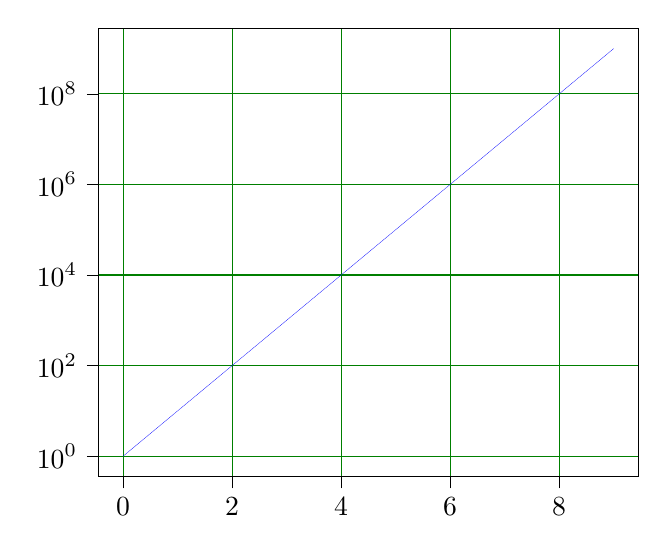
\begin{tikzpicture}

\definecolor{green01270}{RGB}{0,127,0}

\begin{axis}[
log basis y={10},
tick align=outside,
tick pos=left,
x grid style={green01270},
xmajorgrids,
xmin=-0.45, xmax=9.45,
xminorgrids,
xtick style={color=black},
y grid style={green01270},
ymajorgrids,
ymin=0.35481339, ymax=2.8183829e+09,
yminorgrids,
ymode=log,
ytick style={color=black},
ytick={0.01,1,100,10000,1000000,1e+08,1e+10},
yticklabels={
  \(\displaystyle {10^{-2}}\),
  \(\displaystyle {10^{0}}\),
  \(\displaystyle {10^{2}}\),
  \(\displaystyle {10^{4}}\),
  \(\displaystyle {10^{6}}\),
  \(\displaystyle {10^{8}}\),
  \(\displaystyle {10^{10}}\)
}
]
\addplot [ultra thin, blue]
table {%
0 1
1 10
2 100
3 1000
4 10000
5 100000
6 1000000
7 10000000
8 1e+08
9 1e+09
};
\end{axis}

\end{tikzpicture}
